\documentclass{article}
\usepackage[utf8]{inputenc}
\usepackage{amsmath}
\usepackage{graphicx}
\graphicspath{ {./images/} }
\title{BIOS13 - Question 4}
\author{Pham Xuan Huy Nguyen}
\renewcommand\thesection{\alph{section}}
\begin{document}
\maketitle
\section{R function of simulation}
The \textbf{\emph{simulation}} function takes two arguments \textit{pe} as the extinction probability and \textit{ps} as speciation probability, and one optional argument \textit{n} is the number of species in the first period, the default \textit{n} is set as 1.\\
A possible outcome for the function \textit{simulation(0.1,0.2)} is shown below the code part.
\begin{verbatim}
rm(list=ls())
simulation <- function(pe,ps,n) {
  if(missing(n)) {
    x = c(1,rep(0,99)) #If n is not given, then it is set as 1
  } else {
    x = c(n,rep(0,99))
  }
  for (iter in 1:99) {
    temp=0
    if (x[iter]==0) {
      break #At any period, when population reaches 0, stop the loop.
    } else {
      for (i in 1:x[iter]) {
        e = runif(1) # Extinct prob and Speciate prob 
                     # are generated differently randomly for every species
        s = runif(1)
        if (e<=pe){
          temp=temp-1
        } else if (e>pe & s<=ps) {
          temp=temp+1
        } else if (e>pe & s>ps) {
          temp=temp+0
        }
      }
      x[iter+1]=x[iter]+temp
    }
  }
  plot(NA, type='n',xlim=c(0,10),ylim=c(0,max(x)),
    ylab='Number of species',xlab='time (years) x 10^6')
  lines(seq(0.1,10,by=0.1),x) 
  return(x)
}
\end{verbatim}
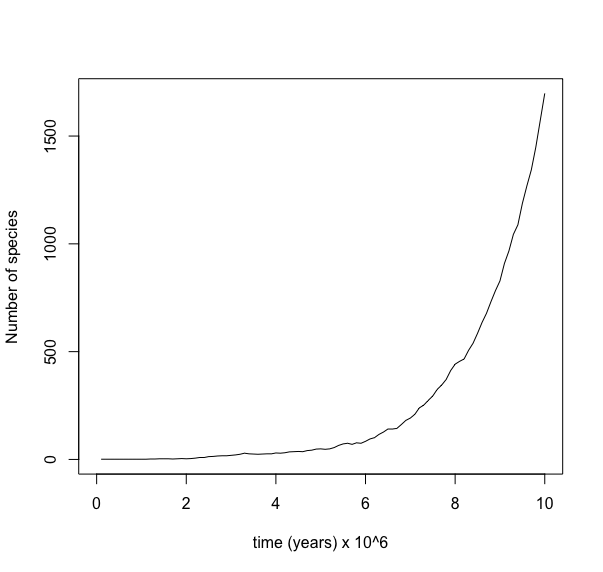
\includegraphics[width=\textwidth]{images/4a.png}
\section{Histogram}
A possible outcome when running the \textit{4b.R} file is shown below the code part.
\begin{verbatim}
rm(list=ls())
simulation <- function(pe,ps,n) {
  if(missing(n)) {
    x = c(1,rep(0,99)) #If n is not given, then it is set as 1
  } else {
    x = c(n,rep(0,99))
  }
  for (iter in 1:99) {
    temp=0
    if (x[iter]==0) {
      break
    } else {
      for (i in 1:x[iter]) {
        e = runif(1)
        s = runif(1)
        if (e<=pe){
          temp=temp-1
        } else if (e>pe & s<=ps) {
          temp=temp+1
        } else if (e>pe & s>ps) {
          temp=temp+0
        }
      }
      x[iter+1]=x[iter]+temp
    }
  }
  return(x)
}

# histogram
sum_of_simulation=0
for (i in 1:1000) {
  sum_of_simulation=sum_of_simulation+simulation(0.1,0.2)
}
hist(sum_of_simulation)
\end{verbatim}
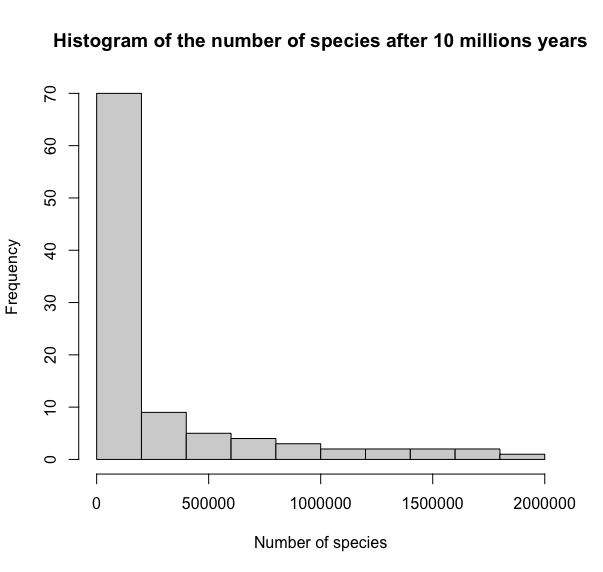
\includegraphics[width=\textwidth]{images/4b.png}
\section{Modification of function for density dependent}
The addition to this function is the \textit{nmax} argument, the maximum number of species. When the number of species is larger or equal to the \textit{nmax}, the \textit{ps} argument is multiple with by the ratio of \textit{nmax} over the number of current population that was multiplied by 1.8. I found that using the number from 1.6 to 1.8 is a good range of number to keep the population approximately equal to \textit{nmax}.  \\
The code \textit{simulation(0.1,0.2,1500)} is used to illustrated to plot.

\begin{verbatim}
rm(list=ls())
simulation <- function(pe,ps,nmax,n) {
  if(missing(n)) {
    x = c(1,rep(0,99))
  } else {
    x = c(n,rep(0,99))
  }
  for (iter in 1:99) {
    temp=0
    if (x[iter]==0) {
      break 
    } else {
      ps_temp=ps*((nmax/1.8)/x[iter])
      pe_temp=pe
      for (i in 1:x[iter]) {
        e = runif(1)
        s = runif(1)
        if (e<=pe_temp){
          temp=temp-1
        } else if (e>pe_temp & s<=ps_temp) {
          temp=temp+1
        } else if (e>pe_temp & s>ps_temp) {
          temp=temp+0
        }
      }
      x[iter+1]=x[iter]+temp
    }
  }
  plot(NA, type='n',xlim=c(0,10),ylim=c(0,max(x)),
       ylab='Number of species',xlab='time (years) x 10^6')
  lines(seq(0.1,10,by=0.1),x) 
  return(x)
}
simulation(0.1,0.2,1500)



\end{verbatim}
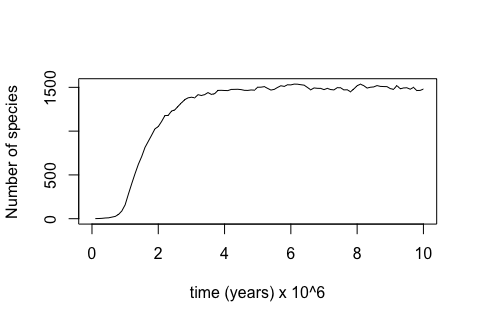
\includegraphics[width=\textwidth]{images/4c.png}
\end{document}
